% The Experiments of the study should be laid out in a series of declarative paragraphs. Only results essential to establish the main points of the work should be included. Often the reporting of the results can be clearer if broken down into subsections. All figures and tables must be cited in the text and must be numbered in the order of their text citation. Figure legends should be self-explanatory, without referring to the text. They should identify the material that is being illustrated, what is shown, and its significance. Each table should be identified by number and should have a title. This section should not include long passages about the rationale of the experiments (which belong in the Introduction), or the methods used (which belong in the Material and Methods), nor should it include justification or discussion of the results (which belong in the Discussion section).
\chapter{Experiments}
\label{sec:experiments}

We perform these experiments to showcase that we can indeed get semantically expressive creations with our proposed formulation.

\section{Environments}

We use two custom environments in our experiments which allow for rich creative expression.

\begin{figure}[h]
    \centering
    \subfloat[\centering ShapeGridWorld]{\fbox{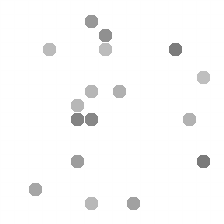
\includegraphics[width=0.4\textwidth]{images/sgw_random.png}}}
    \qquad
    \subfloat[\centering Tangram]{\fbox{
\includegraphics[width=0.4\textwidth]{images/tangram_random.png}}}
    \caption{The environments.}
    \label{fig:environments}
\end{figure}

\subsection{ShapeGridWorld}
\label{sec:sgw}
ShapeGridWorld is a pixel grid environment where the agent can draw on the grid by moving pixels around, either one or all of them at the same time.
This is reminiscent of the pin-board platform used in the free play study conducted by \citet{diggs} (\figref{fig:diggs}).
By setting the pixels in a specific layout, the agent can draw a variety of shapes on the grid.
This environment was adapted from the pixel grid environment used in the work by \citet{rair} with some modifications summarised in the appendix \ref{sec:sgw-details}.

ShapeGridWorld was mostly used in the initial experiments but it later proved to promote noise in CLIP inferences which led to underwhelming results.
To work around the problems, the Tangram environment was developed.

\subsection{Tangram}
\label{sec:tangram}
Tangram is a traditional puzzle game consisting of a canvas and seven geometric shapes -- five right isosceles triangles (two large, one medium, and two small), one square, and one parallelogram, which conventionally have distinct colors.
These shapes can be rotated, flipped, and translated on the canvas.
Even though this is a very simple setup, these pieces can be arranged in very different configurations to create expressive abstract patterns.

This virtual environment was developed specifically for our experiments as it worked around the problems discussed in sections \secref{sec:sparse-rewards} and \secref{sec:inference-noise}, and is a major contribution of this work.
Please refer to appendices \ref{sec:tangram-details} for more details about this environment.

\section{Initial Tests with CLIP}
\label{sec:clip-custom}


\subsection{CLIP on Sketches}
\label{sec:clip-sketches}


\subsection{CLIP on MNIST}
\label{sec:clip-mnist}


\subsection{CLIP on ShapeGridWorld}
\label{sec:clip-sgw}


\subsection{CLIP on Tangram}
\label{sec:clip-tangram}


\subsection{Effect of Resolution}
\label{sec:clip-resolution}


\subsection{Effect of Color and Inversions}
\label{sec:clip-color}


\subsection{Effect of General vs Specific Labels}
\label{sec:clip-labels}



\section{Trajectory Analysis with Random Rollouts}
\label{sec:random-rollouts}
% Problems with CLIP


\subsection{Sparse Rewards} % Suddent changes in rewards
\label{sec:sparse-rewards}


\subsection{Inference Noise} % Confidence in random images
\label{sec:inference-noise}



\section{Initial Simulations on ShapeGridWorld}
\label{sec:sgw-simulations}

\subsection{Partial Completion}
\label{sec:partial-completion}



\section{Improving CLIP Rewards}
\label{sec:improving-rewards}

\subsection{Effect of the Number of Creative Possibilities}
\label{sec:clip-categories}
% categories


\subsection{Comparing CLIP Models}
\label{sec:clip-comparison}


\subsection{Entropy Regularization}
\label{sec:entropy-regularization}
% flatnet


\subsection{Adversarial Performance}
\label{sec:adversarial-performance}


\subsection{Post-hoc Analysis on Rollouts with Closeness Costs}
\label{sec:closeness-rollouts}
% closeness_reward_scale
% closeness_reward_threshold

% Manual ranking and entropy ranking

\subsubsection{Sparse Incremental Closeness Rewards}
\label{sec:sparse-incremental-closeness}


\subsubsection{Sparse Shaped Closeness Rewards}
\label{sec:sparse-shaped-closeness}


\subsubsection{Dense Closeness Rewards}
\label{sec:dense-closeness}


\subsection{Tuning Environment Parameters}
\label{sec:env-hyperparameters}
% render_kwargs.invert
% render_kwargs.color


\subsubsection{ShapeGridWorld}
\label{sec:sgw-parameters}
% width
% x_step
% render_delta
% object_persistency
% max_dist
% control
% control_boundaries


\subsubsection{Tangram}
\label{sec:tangram-parameters}
% flip
% rotate
% x_size
% r_size
% x_step
% object_persistency
% max_dist
% control
% control_boundaries
% staging_boundaries


\subsection{Tuning Controller Hyperparameters}
\label{sec:icem-hyperparameters}
% action_sampler_params.opt_iterations
% action_sampler_params.init_std
% action_sampler_params.elites_size
% num_simulated_trajectories
% horizon
% cost_along_trajectory
% discount_along_trajectory


\subsection{Effect of Target Baseline Regularization}
\label{sec:reg-alpha}
% semantics_alpha_target


\subsection{Effect of Image Baseline Regularization}
\label{sec:reg-beta}
% semantics_beta_image


\subsection{Effect of Temperature}
\label{sec:reg-temperature}
% semantics_model_temperature


\subsection{Effect of Changing Prefix and Suffix}
\label{sec:prefix-suffix}
% label_prefix
% label_suffix


\subsection{Effect of Adding Post-Suffix}
\label{sec:post-suffix}
% Jibberish and adding concepts in post-suffix (WaffleCLIP)
% \cite{waffleclip} found that the exact structure of the phrase, and even tailing it a random string of jibberish, can affect the reward.


\subsection{Effect of Negative Embeddings}
\label{sec:negative-embeddings}


\subsection{Effect of Image Operations}
\label{sec:image-operations}
% Shearing and Hatching



\section{Simulations}
\label{sec:simulations}


\subsection{Effect of RaIR}
\label{sec:effect-rair}
% compression_precision
% 1 / semantics_reward_scale

